\documentclass[fleqn,envcountsame]{LMCS}

\def\doi{8(3:21)2012}
\lmcsheading {\doi}
{1--24}
{}
{}
{Dec.~23, 2011}
{Sep.~20, 2012}
{}
 
\usepackage{tikz}
\usetikzlibrary{shapes}
\usetikzlibrary{snakes}
\usetikzlibrary{arrows} 
\usepackage{mathtools}
\usepackage{stmaryrd}
\usepackage{xspace}
\usepackage{enumerate,hyperref}
\usepackage{amssymb,amsmath}
\usepackage{url}

\makeatletter
\newcommand{\@abbrev}[3]{
  \def\c@a@def##1{
      \if ##1.
        \relax
      \else
        \@ifdefinable{\@nameuse{#1##1}}{\@namedef{#1##1}{#2##1}}
        \expandafter\c@a@def
      \fi
    }
  \c@a@def #3.
}
\@abbrev{bb}{\mathbb}{ABCDEFGHIJKLMNOPQRSTUVWXYZ}
\@abbrev{bf}{\mathbf}{ABCDEFGHIJKLMNOPQRSTUVWXYZabcdefghijklmnopqrstuvwxyz}
\@abbrev{bit}{\boldsymbol}{ABCDEFGHIJKLMNOPQRSTUVWXYZabcdefghijklmnopqrstuvwxyz}
\@abbrev{cal}{\mathcal}{ABCDEFGHIJKLMNOPQRSTUVWXYZ}
\@abbrev{frak}{\mathfrak}{ABCDEFGHIJKLMNOPQRSTUVWXYZabcdefghijklmnopqrstuvwxyz}
\@abbrev{rm}{\mathrm}{ABCDEFGHIJKLMNOPQRSTUVWXYZabcdefghijklmnopqrstuvwxyz}
\@abbrev{scr}{\mathscr}{ABCDEFGHIJKLMNOPQRSTUVWXYZ1234567890}
\@abbrev{sf}{\mathsf}{ABCDEFGHIJKLMNOPQRSTUVWXYZabcdefghijklmnopqrstuvwxyz}
\makeatother

\newcommand{\ot}{\leftarrow}
\newcommand{\Prob}{\ensuremath{\mathrm{Pr}}}
\newcommand{\Val}{\ensuremath{\mathrm{Val}}}
\newcommand{\val}{\ensuremath{\mathrm{val}}}

\newcommand{\cf}{cf.\xspace}
\newcommand{\ea}{\& al.\xspace}
\newcommand{\eg}{e.g.\xspace}
\newcommand{\ie}{i.e.\xspace}

\newcommand{\muc}{-calculus\xspace}
\newcommand{\qmu}{quantitative \muc}

\newcommand{\Qmu}{\ensuremath{Q\mu}\xspace} 

\newcommand{\pzero}{Player~\xspace}
\newcommand{\pone}{Player~\xspace}

\newcommand{\Rinf}{\ensuremath{\mathbb{R}_{\infty}}}
\newcommand{\Qinf}{\ensuremath{\mathbb{Q}_{\infty}}}
\newcommand{\Zinf}{\ensuremath{\mathbb{Z}_{\infty}}}
\newcommand{\Zinfe}{\ensuremath{\mathbb{Z}^{\varepsilon}_{\infty}}}
\newcommand{\setR}{\ensuremath{\mathbb{R}}}
\newcommand{\setQ}{\ensuremath{\mathbb{Q}}}
\newcommand{\setZ}{\ensuremath{\mathbb{Z}}}
\newcommand{\setB}{\ensuremath{\{0,1\}}}
\newcommand{\Pot}{\ensuremath{\calP}}
\newcommand{\Func}{\ensuremath{\mathcal{F}}}
\newcommand{\Diam}{\ensuremath{\Diamond}}
\newcommand{\ol}[1]{\ensuremath{\overline{#1}}}
\newcommand{\mc}{\ensuremath{\mathrm{MC}}} \newcommand{\sem}[1]{\ensuremath{\llbracket#1\rrbracket}}
\newcommand{\semk}[1]{\ensuremath{\llbracket#1\rrbracket^{\calK}}}
\newcommand{\lint}{\ensuremath{\frakI}} \newcommand{\semek}[1]{
  \ensuremath{\llbracket#1\rrbracket_{\lint}^{\calK}}
}
\newcommand{\semsub}[1]{
  \ensuremath{\llbracket#1\rrbracket_{\lint[X \leftarrow f]}^{\calK}}
}

\newcommand{\floor}[1]{\ensuremath{\lfloor #1 \rfloor}}
\newcommand{\ceil}[1]{\ensuremath{\lceil #1 \rceil}}
\newcommand{\intervals}{\ensuremath{\calI(\Rinf)}}
\newcommand{\intervalsplus}{\ensuremath{\calI(\Rinf^{\geq 0})}}
\newcommand{\labels}{\ensuremath{\lambda}}
\newcommand{\successor}{\ensuremath{\mathrm{succ}}}
\newcommand{\coeff}{\ensuremath{\delta}} \newcommand{\indexi}{\ensuremath{\iota}}
\newcommand{\strat}{\ensuremath{\sigma}} \newcommand{\pay}{\ensuremath{\mathrm{p}}} \newcommand{\di}{\ensuremath{\mathrm{d}}} \newcommand{\dih}{\ensuremath{\mathrm{d^*}}}
\newcommand{\corr}{\ensuremath{\mathrm{c}}}
\newcommand{\dleft}{\ensuremath{\mathrm{d}_l}}
\newcommand{\dright}{\ensuremath{\mathrm{d}_r}}
\newcommand{\loc}{\ensuremath{\mathrm{loc}}} \newcommand{\var}{\ensuremath{\mathrm{var}}} \renewcommand\epsilon{\varepsilon}
\renewcommand\phi{\varphi}
\newcommand{\siff}{\Leftrightarrow} \newcommand{\nin}{\ensuremath{\not \in}}
\renewcommand{\max}{\mathrm{max}}
\newcommand{\cupdot}{\mathbin{\dot{\cup}}}
\newcommand{\closedots}{\mathinner{\!\ldotp\!\ldotp\!\ldotp\!}}

\pagestyle{plain} 


\begin{document}

\title[Model Checking the Quantitative -Calculus on
  Linear Hybrid Systems]{Model Checking the Quantitative -Calculus on
  Linear Hybrid Systems}
\author[D.~Fischer]{Diana~Fischer\rsuper a}
\address{{\lsuper a}Mathematische Grundlagen der Informatik, RWTH Aachen University}
\email{fischer@logic.rwth-aachen.de}

\author[\L.~~Kaiser]{\L{}ukasz~Kaiser\rsuper b}
\address{{\lsuper b}LIAFA, CNRS \& Universit{\'e} Paris Diderot -- Paris 7}
\email{kaiser@liafa.univ-paris-diderot.fr}

\thanks{Authors were supported by DFG~AlgoSyn~1298 and
  ANR~2010~BLAN~0202~02~FREC}

\keywords{hybrid systems, model checking, -calculus, quantitative logics,
  games}
\subjclass{D.2.4, F.4.1}

\begin{abstract}
We study the model-checking problem for a quantitative
extension of the modal -calculus on a class of hybrid systems.
Qualitative model checking has been proved decidable and implemented for
several classes of systems, but this is not the case for quantitative
questions that arise naturally in this context. Recently, quantitative
formalisms that subsume classical temporal logics and allow
the measurement of interesting quantitative phenomena were introduced.
We show how a powerful quantitative logic, the quantitative -calculus, can
be model checked with arbitrary precision on initialised linear hybrid systems.
To this end, we develop new techniques for the discretisation of continuous
state spaces based on a special class of strategies in model-checking games
and present a reduction to a class of counter parity games.
\end{abstract}

\maketitle

\section{Introduction}

Modelling discrete-continuous systems by a hybrid of a discrete transition
system and continuous variables which evolve according to a set of
differential equations is widely accepted in engineering.
While model-checking techniques have been applied to verify safety, liveness
and other temporal properties of such systems \cite{ACHHHNOSY95,HHM99,HKPV95},
it is also interesting to infer quantitative values for certain queries.
For example, one may not only want to check that a variable of a system
does not exceed a given threshold, but also to compute the maximum value
of the variable over all runs, checking whether any such threshold exists.

Thus far, quantitative testing of hybrid systems has only been done
by simulation, and hence lacks the strong guarantees which can be given
by model checking. In recent years, there has been a strong interest
in extending classical model-checking techniques and logics to the quantitative
setting. Several quantitative temporal logics have been introduced,
see \eg  \cite{Alfaro03,AlfaroFS04,AlfaroM04,FGK10,seidl07,Hugo07,McIver},
together with model-checking algorithms for simple classes of systems,
such as finite transition systems with discounts. Still, none of those
systems allowed for dynamically changing continuous variables.
We present the first model-checking algorithm for a non-stochastic quantitative
temporal logic on a class of hybrid systems.
The logic we consider, the quantitative -calculus \cite{FGK10},
is based on a formalism first introduced in \cite{AlfaroFS04}.
It properly subsumes the standard -calculus, \cf \cite{BradfieldS01}, and
thus also CTL and LTL.
Therefore the present result, namely that it is possible to
model check quantitative -calculus on initialised linear
hybrid systems, properly generalises a previous result on
model checking LTL on such systems \cite{HHM99,HKPV95}, which is
one of the strongest model-checking results for hybrid systems.

The restriction to initialised linear systems is made because verification
of temporal properties over general hybrid systems is undecidable. This
holds even for linear systems, thus one must pick an appropriate abstraction
of the system. An established and very well-studied way to do this is to
first approximate the continuous behaviour of the variables by linear
behaviour in a finite number of intervals.
This method, applied to a number of functions  that
evolve according to a set of arbitrary differential equations
, generates a set of disjoint intervals
 with  and
a set of linear coefficients  such that in  it is
approximately true that , \ie the
derivative . There are several
ways to generate such linear approximations of solutions of differential
equations and, depending on the method in question, one can obtain various
kinds of error bounds for the respective classes of functions.
We do not investigate these issues (or other approximation methods) here,
but focus instead on the linear system obtained. 

As stated above, even simple
qualitative verification problems are undecidable for general hybrid systems.
This remains true even after the natural approximation by a linear system.
Hence, one more assumption is made, namely that if the speed of evolution of a
variable changes between discrete locations then also the variable is reset
on that transition. Systems with this property, called \emph{initialised}
linear systems, are -- besides o-minimal systems \cite{LPS00,BBC07} and their
recent extensions \cite{VPVD08} -- one of the largest classes of hybrid systems
with decidable temporal logic \cite{HKPV95}.
Observe that when an arbitrary hybrid system is approximated by a linear one,
one can \emph{try} to directly obtain an initialised system by computing
boundary values \cite{HHW96}. This can be done by either assuring that discrete
transitions are taken only at the borders of the intervals , or by taking
a finer subdivision of the intervals to increase the precision of coordination
between the discrete and the continuous part of the system. Note that, even
though this procedure has been implemented in model-checking programs, it is
only a heuristic -- it necessarily fails for general systems for which the
model-checking problem is undecidable.

The logic we study is quantitative -- it allows to express properties involving
suprema and infima of values of the considered variables during runs that
satisfy various temporal properties, \eg to answer
``what is the maximal temperature on a run during which a safety condition
holds?''. To model check formulae of the quantitative -calculus,
we follow the classical parity game-based approach
and adapt some of the methods developed in the qualitative
case and for timed systems. To our surprise, these methods turned out
not to be sufficient and did not easily generalise to
the quantitative case. As we will show below, the quantitative systems we study
behave in a substantially different way than their qualitative counterparts.
We overcome this problem by working directly with a quantitative
equivalence relation, roughly similar to the region graph for timed automata,
and finally by exploiting a recent result on counter parity games.

\textbf{Organisation.}
The organisation of this paper follows the reductions needed to model check
a formula  over a hybrid system . 
In Section \ref{sec_hybrid}, we introduce the necessary notation,
the systems and the logic. Then, we present
an appropriate game model in Section \ref{sec_ipg} and show how to 
construct a model-checking game  for the system and the formula.
In Section \ref{sec_basic}, we transform the interval games constructed for
arbitrary initialised linear hybrid systems to flat games, where the linear
coefficients are always . In Section \ref{sec_ds}, we show how the strategies
can be discretised and still lead to a good approximation of the original game.
Finally, in Section \ref{sec_pushdown}, we reduce the problem to counter
parity games and exploit a recent result to solve them.
To sum up, the steps taken are depicted below.



\section{Hybrid Systems and Quantitative Logics} \label{sec_hybrid}
We denote the real and rational numbers and integers extended with both
 and  by ,  and  respectively.
We write  and  for all open or closed
intervals over  with endpoints in  and .

\begin{defi}
A \emph{linear hybrid system over  variables},
,
is based on a directed graph , consisting of a set of locations 
and transitions . The labelling function
 assigns to each transition
a finite set of labels. The set  of \emph{transition labels}
consists of triples , where the vector
 (with  for
) represents the constraints each of the variables
needs to satisfy for the transition to be allowed, the interval
 represents the possible period of time
that elapses before the transition is taken,
and the reset set  contains the indices of the
variables that are reset during the transition, 
\ie  means that  is set to zero.
For each  of the finite index set ,
the function  assigns to each location
the value of the static quantitative predicate .
The function  assigns to each location
and variable  the coefficient  such that the variable evolves
in this location according to the equation .
\end{defi}

Please note that although we do not explicitly have any invariants
(or constraints) in locations, we can simulate them by choosing either
the time intervals or variable constraints on the outgoing transitions
accordingly. If the values of predicates and labels range over 
or  instead of , we talk about linear hybrid systems
over  and , respectively. 

The \emph{state} of a linear hybrid system  is a location
combined with a valuation of all  variables, .
For a state  we say that a transition
 is \emph{allowed} by a label 
if  (\ie if  for all ).
We say that a state  is a successor of ,
denoted , when there is a transition ,
allowed by label , such that  for all  and
there is a  such that  where 
 for all .
A run of a linear hybrid system starting from location  is
a sequence of states  such that 
and  for all . Given two states  and
 and a reset set  we denote by
 the increase of the non-reset variables that occurred during the
transition, \ie  for some  where
 and . 

\begin{defi}
A linear hybrid system  is \emph{initialised} if for each
 and each variable  it holds that if 
 then  for .
\end{defi}

Intuitively, an initialised system cannot store the value of a variable
whose evolution rate changes from one location to another.

\begin{exa}
To clarify the notions we use, we consider a variant of a standard example 
for a linear hybrid system, the leaking gas burner.

\begin{figure}
\begin{center}
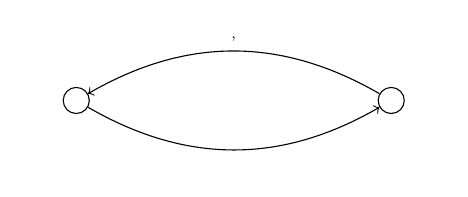
\begin{tikzpicture}
\node[draw,circle] (a) at (-2, 0) {};
\node[] () at (-2, 0.75) {{\small{}}};
\node[] () at (-2.5, -0.75) {\emph{\small{}}};
\node[draw, circle] (b) at (2, 0) {};
\node[] () at (2, 0.75) {{\small{}}};

\node[] () at (2.5, -0.75) {\emph{\small{}}};
\path (a) edge[bend right,->] node[above] {{\tiny{}}}
node[below] {{\tiny{}}} (b);
\path (b) edge[bend right,->] node[below] {{\tiny{}}}
  node[above] {{\tiny{,}}} (a);
\end{tikzpicture} 
\end{center}
\caption{Leaking gas burner LHS  (not initialised)}\label{leaking-not-in}
\end{figure}

Our version is depicted in Figure \ref{leaking-not-in}. 
This system represents a gas valve that can leak gas to a burner, so it has
two states: , where the valve is open (and leaking gas) and  where
it is closed. This is also indicated by a qualitative predicate  that
has the value  if the gas is leaking (in location ) and
 otherwise.
The system has two variables. The first variable, , is a clock
measuring the time spent in each location, and is reset on each transition,
\ie after each discrete system change. The variable  is a stop watch
and measures the total time spent in the leaking location.
Thus, this system is not initialised.
The time intervals on the transitions control the behaviour of the system.
On the transition  there are no restrictions on the variables, but
we are only allowed to choose a time unit from , \ie we can stay a
maximum of one time unit in location . On the transition  there 
is a restriction on the value of , it has to have a value between 30
and 40 for this transition to be allowed, while there is no restriction on
the choice for the time unit (of course, this could also be modelled the other
way around).
Intuitively, the time intervals indicate that the gas valve will
leak gas for a time interval between 0 and 1 seconds and 
then be stopped and that it can only leak again after
at least 30 time units.\\

In Figure \ref{leaking}, we show an initialised version of the leaking gas burner.
The only difference is that  is not a stop watch anymore but a normal
clock. Since now both variables are just clocks (which means that their
evolution rates are one everywhere), the system is trivially initialised.

\begin{figure}
\begin{center}
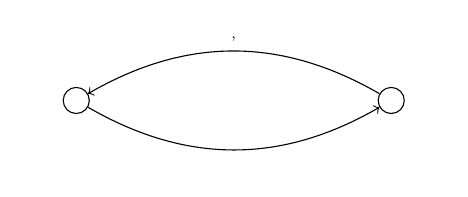
\begin{tikzpicture}
\node[draw,circle] (a) at (-2, 0) {};
\node[] () at (-2, 0.75) {{\small{}}};
\node[] () at (-2.5, -0.75) {\emph{\small{}}};
\node[draw, circle] (b) at (2, 0) {};
\node[] () at (2, 0.75) {{\small{}}};
\node[] () at (2.5, -0.75) {\emph{\small{}}};
\path (a) edge[bend right,->] node[above] {{\tiny{}}}
node[below] {{\tiny{}}} (b);
\path (b) edge[bend right,->] node[below] {{\tiny{}}}
  node[above] {{\tiny{,}}} (a);

\end{tikzpicture} 
\end{center}
\caption{Leaking gas burner LHS  (initialised)}\label{leaking}
\end{figure}
\end{exa}

\subsection{Quantitative -Calculus}
In this section, we present a version of the quantitative -calculus first
introduced in \cite{FGK10}.
The version we use here is additive and includes variables. It is evaluated on
linear hybrid systems.

\begin{defi}
Given sets of fixpoint variables , system variables  and predicates ,
the formulae of the \emph{quantitative \muc (\Qmu) with variables}
are given by the EBNF grammar:

where , and in the cases
 and , the variable  must appear positively
in , \ie under an even number of negations.
\end{defi}


Let .
Given an interpretation ,
a variable , and a function , we denote by
 the interpretation ,
such that  and 
for all .

\begin{defi}
Given a linear hybrid system
 and an interpretation
, a -formula yields a valuation
function  defined in the following standard
way for a state .
\begin{iteMize}{}
\item , 
      , and
      , 
\item  and
      ,
\item  and
      ,
\item ,\\
  .
\end{iteMize}
\end{defi}

\noindent For formulae without free variables we write 
rather than .

Please note that the inclusion of variables does not fundamentally 
change the semantics of \qmu. The \qmu in \cite{FGK10} is evaluated
on quantitative transition systems. Here, a formula is evaluated on
the state graph of a linear hybrid system, rather than the system itself.
Intuitively, a linear hybrid system is a compact representation
of an infinite quantitative transition system (its state graph).
Thus, many properties of the \qmu from \cite{FGK10} remain true.
For example, to embed the classical -calculus in \qmu one must
interpret \emph{true} as  and \emph{false} as .

\begin{exa}
The formula  evaluates to the supremum of
the values of  on all runs from some initial state:
e.g. to  if evaluated on the simple initialised
leaking gas burner model. To determine the longest period of time
during which the gas is leaking we use the formula
, which evaluates to  on
the initial state  in our example.
\end{exa}


The remainder of this paper is dedicated to the proof of our following
main result which shows that  can be approximated
with arbitrary precision on initialised linear hybrid systems.

\begin{thm} \label{mainthm}
Given an initialised linear hybrid system , a \qmu formula 
and an integer , it is decidable whether ,
, or else a number  can be computed
such that .
\end{thm}

In other words, for every  we can approximate 
within . We formulated the theorem above using  because it
makes the representation of  precise, so we can provide a complexity
bound: Given on input the system , the formula  and , we will
show how to compute the number  (or output ) in \textsc{8EXPTIME}.


\section{Interval Games}\label{sec_ipg}

In this section, we define a variant of quantitative parity games
suited for model checking \Qmu on linear hybrid systems.
As mentioned above, a linear hybrid system can be seen as a compact 
representation of an infinite quantitative transition system. 
Similarly, a parity game that is played on a linear hybrid
system can be viewed as a compact, finite description of an
infinite quantitative parity game, as defined in \cite{FGK10}.

\begin{defi} \label{def-ipg}
An \emph{interval parity game} (IPG)
,
is played on a LHS  (without predicates) and
 is divided into positions of either \pzero or 1. 
The transition relation   describes possible
moves in the game which are labelled by the function
.
The function  assigns to each
position the index of a variable and a multiplicative and additive factor,
which are used to calculate the payoff if a play ends in this position.
The priority function 
assigns a priority to every position.
\end{defi}

Please note that interval parity games are played on linear hybrid systems without any quantitative predicates,
\ie the set of of predicates is empty and therefore omitted.

A \emph{state}  of an interval game
is a position in the game graph together with a variable assignment for
all  variables. 
A state  is a successor of  if it is a successor
in the underlying LHS, \ie if .
We use the functions  and  to 
access the components of a state.
For a real number , we denote by  and  
We call  the state set  where player 
has to move and .

\textbf{How to play.}
Every play starts at some position  with all variables set to ,
\ie the starting state is .
For every state , player 
chooses an allowed successor state  and the play
proceeds from . If the play reaches a state  such that
 it ends, otherwise the play is infinite.

Intuitively, the players choose the time period they want to spend
in a location before taking a specified transition.
Note that in this game every position could possibly be a terminal
position. This is the case if it is not possible to choose a time period
from the given intervals in such a way that the respective constraints
on all variables are fulfilled.

\textbf{Payoffs.}
The outcome  of a finite play ending in 
 where  is
.
To improve readability, from now on we will simply write 
 in this case.
The outcome of an infinite play depends only on the lowest priority seen
infinitely often in positions of the play. We will assign the value
 to every infinite play, where the lowest priority seen infinitely
often is odd, and  to those where it is even.


\textbf{Goals.}
The two players have opposing objectives regarding the outcome of the play.
\pzero wants to maximise the outcome, while \pone wants to minimise~it.

\textbf{Strategies.} 
A strategy for player  is a function
 with .
A play  is \emph{consistent with a strategy} 
for player , if  for every  such that
.
For strategies  for the two players, 
we denote by  the unique
play starting in state  which is consistent with both  and
.

\textbf{Determinacy.} 
A game is \emph{determined} if, for each state , the highest outcome
\pzero can assure from this state and the lowest outcome \pone can assure
coincide,

where  are the sets of all possible strategies 
for \pzero, \pone and the achieved outcome is called the 
\emph{value of  at }.

We say that the interval game is over  or  if both
the underlying LHS and all constants in 
are of the respective kind. Please note that this does
not mean that the players have to choose their values from  or
, just that the endpoints of the intervals and constants
in the payoffs are in those sets.

Intuitively, in a play of an interval parity game, the players choose
successors of the current state as long as possible.
\begin{exa}
In Figure \ref{ipg}, we show a simple example of an interval parity game.
Positions of \pzero are depicted as circles and positions of \pone
as boxes. To keep things simple, there is just one clock variable, 
, all constraints are trivially true and the reset
sets are empty, so we label the transitions only with the time intervals
that the players can choose from. 
The priorities are depicted next to the nodes for non-terminal
positions and the evaluation function above the terminal position (in general, also
positions with outgoing edges could be terminal, however in this example this is
not possible as there are no constraints on the variable).

A play of this system starting at node  could end after two
moves in position , if \pone decided to move there (he also has the choice to
move down). 
The payoff of this play would then
depend only on the choice that \pzero made in the first move, for example . 
Then the payoff would be
 (as in this 
play, the second time interval only permits the choice ).

If \pone would move down instead
of ending the play and the play would loop infinitely often in the cycle 
at the bottom, the least priority that occurs infinitely often would 
determine the outcome of the play; in this case it would be 0 at  and therefore
the payoff would be .
\end{exa}
\begin{figure}[h]\label{ipg}
\begin{center}
\begin{tikzpicture}

\node [circle,draw] (a) at (0,1) {};
\node [circle] (a1) at (1.3,1) {\small{}};

\node [rectangle,draw,minimum size =0.6cm] (b) at (0,-0.5) {};
\node [rectangle] (b1) at (1.3,-0.5) {\small{}};

\node [rectangle,draw, minimum size =0.6cm] (c) at (-2,-0.5) 
  {\small{{}}};
\node [rectangle] (c1) at (-2.5,0.1) 
  {\small{{}}};

\node [circle,draw] (d) at (0,-2) {};
\node [circle] (d1) at (-1.3,-2) {\small{}};

\node [circle,draw] (e) at (-2,-3) {};
\node [circle] (e1) at (-3.3,-3) {\small{}};

\node [circle,draw] (f) at (2,-3) {};
\node [circle] (f1) at (3.3,-3) {\small{}};

\path[->] (a) edge []node[right] {{\tiny{}}} (b);
\path[->] (b) edge []node[above] {{\tiny{}}} (c);

\path[->] (b) edge []node[right] {{\tiny{}}} (d);
\path[->] (d) edge []node[above] {{\tiny{}}} (e);
\path[->] (f) edge []node[above] {{\tiny{}}} (d);
\path[->] (e) edge []node[above] {{\tiny{}}} (f);
\path[->] (f.north) edge [bend right]node[right] {{\tiny{}}} (b.east);
\end{tikzpicture}
\end{center}
\caption{Simple interval parity game} 
\end{figure}

We already mentioned that an interval parity game can be seen
as a representation of a quantitative parity game, now we 
want to describe this formally.
We use the notion from \cite{FGK10} and define,
for an IPG with  variables
,
the corresponding infinite quantitative parity game without discounts

with  iff  is a successor of  as above,
 and
 iff
.
The notions of plays, strategies, values and determinacy 
for the IPG  are defined exactly as the ones for
the quantitative parity game  in \cite{FGK10}.
In particular, it follows from the determinacy of
quantitative parity games that also interval parity games
are determined.

\subsection{Model-Checking Games for \Qmu} \label{subsec_mc}

A game  is a model-checking game for a formula  and
a system , if the value of the game starting from  is
exactly the value of the formula evaluated on  at .
In the qualitative case, that means, that  holds in  if
\pzero wins in  from~. For a linear hybrid system 
and a \Qmu-formula , we construct an IPG
 which is the model-checking game for  on .

The full definition of  closely follows the construction
presented in~\cite{FGK10} and is presented below.

Intuitively, the positions are pairs consisting of a subformula
of  and a location of . 
Which player moves at which position depends on the outermost 
operator of the subformula. At disjunctions \pzero moves
to a position corresponding to one of the disjuncts and from 
 to  where 
, and \pone makes analogous
moves for conjunctions and . From fixed-point variables the play
moves back to the defining formula and the priorities
of positions depends on the alternation level of fixed points, 
assigning odd priorities to least fixed points and even priorities 
to greatest fixed points.

\begin{defi}
For a linear hybrid system 
and a \Qmu-formula  in negation normal form, the interval game 

which we call the \emph{model-checking game} for  and ,
is constructed in the following way, similar to the standard construction
of model-checking games for the -calculus (c.f. \cite{FGK10}).
\end{defi}

\textbf{Positions.}
The positions of the game are pairs ,
where  is a subformula of , and
 is a location in the LHS .
Positions  where the top operator
of  is , or  belong to \pone and
all other positions belong to \pzero.
A state in the game is denoted by , where 
is the position and  is the variable assignment of
the location  in the underlying linear hybrid system .

\textbf{Moves.} 
Positions of the form  and 
are terminal positions.
From positions of the form ,
resp. , one can move to 
 or to  .
Positions of the form  have
either a single successor  in case  is a terminal 
location in , or one successor  for every
. Analogously, positions of the form 
have a single successor  if ,
or one successor  for every  otherwise.
The moves corresponding to system moves  are labelled
accordingly with , all other 
moves are labelled with the empty label 
which indicates that no time passes, there are no constraints on the variables
and no variable is reset.
Fixed-point positions , resp. 
have a single successor .
Whenever one encounters a position where the fixed-point variable stands alone,
\ie , the play goes back to the corresponding definition,
to .

\textbf{Payoffs.} 
The function  assigns 
to all positions ,  to all
positions 
and  to positions .
To discourage the players from ending the game at any other position
than a terminal one,  assigns all other positions
outcome  for \pzero's positions or 
for \pone's positions.
The payoff  of a play  is calculated
using  and the priorities as stated before.

\textbf{Priorities.} 
The priority function  is defined as in the classical case
using the alternation level of the fixed-point variables,
see \eg \cite{Graedel03}.
Positions  get a lower priority
than positions  if  has a lower alternation level than .
The priorities are then adjusted to have the right parity, such that
an even value is assigned to all positions  where  is a 
-variable and an odd value to those where  is a -variable.
The maximum priority, equal to the alternation depth of the formula,
is assigned to all other positions.

\begin{exa}
We continue our example of the leaking gas burner and present in
Figure \ref{fig-mcgame-example} the model-checking
game for the previously introduced system and formula.
In this interval parity game, ellipses depict positions of \pzero and rectangles
those of \pone. In this game, all priorities are odd (and therefore
omitted), \ie infinite plays are bad for \pzero.
There is only one position with a constraints on variable  and
in only two positions a choice about the time that passes can be made.
Both of these positions belong to \pzero in this example and are labelled
with the corresponding intervals below (and in both  is also reset).
In terminal nodes, either the variable  or the predicate
 is evaluated for the payoff (this choice can be made by \pone in this example).
The value of the game is , as is the value of the formula on the
system starting from either node, and an optimal strategy for
\pzero is picking  from  and then leaving the cycle
where \pone is forced to choose between the evaluation of
 or  at . Since he is minimising, he will choose
to evaluate .

\begin{figure}
\begin{center}
\begin{tikzpicture}[scale=0.75] \small
\node [ellipse,draw,inner sep=2pt] (a) at (0,2.5)
  {};
\node [ellipse,draw] (b) at (0,1) 
  {};
\node [draw] (e) at (-4,1) {};
\node [ellipse,draw] (f) at (-4, 2.5) {{}};
\node [ellipse,draw] (g) at (-4,-0.5) {{}};
\node [ellipse, draw] (x) at (0,-0.5) {};
\node [ellipse,draw] (d) at (0,-2) {};
\path[->] (a) edge []node {} (b);
\path[->] (b) edge []node {} (x);
\path[->] (x) edge []node[right] {{}} (d);
\path[->] (b) edge []node {} (e);
\path[->] (e) edge []node {} (f);
\path[->] (e) edge []node {} (g);
\node [ellipse,draw,inner sep=2pt] (a2) at (5,-2)
  {};
\node [ellipse,draw] (b2) at (5,-0.5)
  {};
\node [ellipse, draw] (x2) at (5,1) {};
\node [ellipse,draw] (d2) at (5,2.5) {};
\node [draw] (e2) at (9,-0.5) {};
\node [ellipse,draw] (f2) at (9, 1) {{}};
\node [ellipse,draw] (g2) at (9,-2) {{}};
\path[->] (a2) edge []node {} (b2);
\path[->] (b2) edge []node {} (x2);
\path[->] (x2) edge []node[right] {{}} (d2);
\path[->] (b2) edge []node {} (e2);
\path[->] (e2) edge []node {} (f2);
\path[->] (e2) edge []node {} (g2);
\path[->] (d) edge []node {} (a2);
\path[->] (d2) edge []node {} (a);
\end{tikzpicture}
\end{center}
\caption{Model-checking game for  on initialised leaking gas burner.}
\label{fig-mcgame-example}
\end{figure}

\end{exa}


It has been shown in \cite{FGK10} that quantitative parity games of any size
are determined and that they are model-checking games for \Qmu. These results
translate to interval parity games and we can conclude the following.

\begin{thm} \label{mccorrect}
Every interval parity game is determined and
for every formula  in \Qmu, linear hybrid system ,
and a location  of , it holds that

\end{thm}

\begin{proof}
Determinacy of an interval parity game  follows directly from
the determinacy of the infinite QPG  used to define .

Let  be a \Qmu-formula and  a linear hybrid system.
Let  be the state graph of , where 
is the set of all states, and  iff 
in . Let  be the quantitative
transition system with predicates  where .
Let us also rewrite the formula  into a formula without 
variables, , by replacing each occurrence of  by the 
corresponding .

Applying the model-checking Theorem 12 from \cite{FGK10} we conclude
that for all  it holds
,
\ie that  is the model-checking game for
 and . Finally, by definition of IPGs on the one hand and
the semantics of  on the other, it follows that for all 

~\\ \vskip -4.2em
\end{proof}

\section{Basic Properties of Interval Games}\label{sec_basic}
In this section, we first give a brief example that illustrates the difference between
interval games and timed games. Then, we show how to transform an initialised interval game over 
 into an easier game over  in which the all evolution rates are one.

At first sight, interval games seem to be very similar to
timed games. Simple timed games are solved by playing
on the region graph and can thus be discretised.
To stress that quantitative payoffs indeed make a difference,
we present in Figure \ref{fig-game-half-example} an initialised interval parity 
game with the interesting property that it is not optimal to play integer
values, even though the underlying system is over . This simple game
contains only one variable (a clock) and has no constraints on this variable
in any of the transitions, so only the time intervals are shown.
Also, as infinite plays are not possible, the priorities are omitted,
as well as the indices of non-terminal positions (they are chosen to be
unfavourable for the current player such that she has to continue playing). 
The payoff rule specifies the outcome of a play 
ending in  as  and in  as .
This game illustrates that it may not be optimal to 
play integer values since choosing time  in the first move 
is optimal for \pzero. This move guarantees an outcome of 
which is equal to the value of the game.

\begin{figure}[h]
\begin{center}
\begin{tikzpicture}[scale=1]
\small
\node[draw,circle] (v0) at (0, 2.2) {};
\node[draw] (v1) at (0, 1) {};
\node[draw,circle](e1) at (-2, 1) {};
\node[]() at (-2, 0.25) {\small{}};
\node[draw,circle](e2) at (2, 1) {};
\node[]() at (2, 0.25) {\small{}};
\path[->] (v0)  edge node[right] {\tiny{}} (v1);
\path[->] (v1)  edge node[above] {\tiny{}} (e1);
\path[->] (v1)  edge node[above] {\tiny{}} (e2);
\end{tikzpicture}
\end{center}
\caption{Game with integer coefficients and non-integer value.}
\label{fig-game-half-example}
\end{figure}

\subsection{Flattening Initialised Interval Games} \label{subsec_flat}
So far, we have considered games where the values of variables can change at
different rates during the time spent in locations. In this section,
we show that for initialised games it is sufficient to look at easier
games where all rates are one, similar to timed games but with more
complex payoff rules. We call these games flat and show that for every 
initialised IPG we can construct a flat IPG with the same value.
To do so, we have to consider the regions where the coefficients do not
change and rescale the constraints and payoffs accordingly.

For an interval , we denote by 
and  the intervals  and 
respectively, and do analogously for open intervals. 

\begin{defi}
An interval parity game 

is \emph{flat} if and only if 
for all  and .
\end{defi}

\begin{lem} \label{flat}
For each initialised interval parity game  there exists
a flat game  with the same value.
\end{lem}

\begin{proof}
Let 
be an initialised interval parity game.
We construct a corresponding flat game 
 in the following way:
For a position  and each variable , such that 
,  and an outgoing edge  with 
we have in the corresponding flat game:
\begin{iteMize}{}
\item 
\item 
\item 
\end{iteMize}
Note that we only change the functions  and .
We will show that for every play  from a starting state  consistent
with  and , we can construct strategies , ,
such that  visits the same locations as  and
. Before we proceed with the proof, notice that it is
essential that  is an initialised game. Intuitively, the value of 
in  is the value of  in  divided by the coefficient 
of the current position. When the position changes, it is thus crucial that
 does \emph{not} change, except if  is reset -- exactly what is
required from an initialised game.

The proof proceeds by induction on the length of the plays.
First, if  is a state belonging to \pzero and
 and , then in 
we define , where , such that
 for any .
Since  is allowed in , this means that for all
, we have
. It follows that

for all  and therefore  is allowed in .
Also  and therefore the payoff is
equal to .

Let  and  be finite histories in  and
, such that they visit the same locations and .
Then, if  is a state belonging to \pzero and
 and ,
then in  we define , where
, such that  where 
for any .
Since  is allowed in , this means that for
all , .
As  for
all , we get that  is allowed in .
Also  and therefore the payoff is equal
to .

The cases for \pone are analogous. Note that, for infinite plays,
we also have the same payoff, since for the payoff of infinite games only
the locations (and their priorities) matter. Since we can construct, for
each pair of strategies in , the corresponding strategies in ,
and those yield a play with the same payoff, the values of the two games
are equal.
\end{proof}

Consequently, from now on we only consider flat interval parity games and
therefore omit the coefficients, as they are all equal to one.


\subsection{Multiplying Interval Games}\label{subsec_mult}

\begin{defi}
For a flat IPG  and
a value , we denote by
 the IPG where 
 iff  
for all , and   iff
 with  and
 for all .
\end{defi}

Intuitively, this means that all endpoints in the time intervals (open and closed),
and the constraints, and all additive values in the payoff function 
are multiplied by . The values of  are also equal to
the values of  multiplied by .

\begin{lem} \label{mult_games}
For every IPG  over  and  it holds in all states
 that .
\end{lem}

\begin{proof}
We denote by  the strategy with 
 iff 
The mapping of  with strategies for both players  and 
to  with  and  is a bijection 
(in the reverse direction take ). We also have 

where  which is equal to 

for all finite plays . Therefore, we know that 
 
and the same holds for the supremum and thus we get the desired result.
\end{proof}

Note that all multiplicative factors in  are the same in  and
in . Moreover, if we multiply all constants in  in a game
 (both the multiplicative and the additive ones) by a positive value ,
then the value of  will be multiplied by , by an analogous argument as
above. Thus, if we first take  as the least common multiple of all denominators
of multiplicative factors in  and multiply all  constants as above,
and then take  as the least common multiple of all denominators of endpoints
in  the intervals and additive factors in the resulting game  and build
, we can conclude the following.

\begin{cor} \label{mult_games_col}
For every finite IPG  over , there exists an IPG  over  and
 such that .
\end{cor}

From now on we assume that every IPG we investigate is a flat game over 
when not explicitly stated otherwise. 


\section{Discrete Strategies} \label{sec_ds}

Our goal in this section is to show that it suffices to use a simple kind
of (almost) discrete strategies to approximate the value of flat 
interval parity games over .
To this end, we define an equivalence relation between states
whose variables belong to the same  intervals. This equivalence,
resembling the standard methods used to build the region graph from
timed automata, is a technical tool needed to compare the values of
the game in similar states. 

We use the standard meaning
of  and , and denote by  the number 
and by  the pair . Hence, when writing
, we mean that  and  lie in between the same integers.
Note that if  then  implies that .

\begin{defi}
We say that two states  and  in an IPG are equivalent, ,
if they are in the same location, , and for all
:
\begin{iteMize}{}
\item , and
\item if  then .
\end{iteMize}
\end{defi}

Intuitively, all variables lie in the same integer intervals and the order
of fractional parts is preserved. In particular, it follows that all
integer variables are equal.
The following technical lemma allows for the shifting of moves between -states.

\begin{lem} \label{shift-move}
Let  and  be two states in a flat IPG over  such that .
If a move from  to  is allowed by a label ,
then there exists a state , the move to which from  is allowed by
the same label  and .
\end{lem}


\begin{proof}
If  then let .
As , the same constraints are satisfied by  and  and thus
the move from  to  is allowed by the same label.

If  then let  be the increment
chosen during the move. If  we let , the conditions
follow from the assumption that  again.

If , let  be the index of a non-reset variable
with the smallest fractional part in , i.e.
 for all .
To construct , we must choose  with  which makes
 the one with smallest fractional part. 

\emph{Case 1}: .\\
  In this case, for all non-reset variables , holds
  , intuitively meaning
  that no variable ``jumped'' above an integer due to .
  Let  be the variable with maximum fractional part in 
  (and thus, by definition of , also in  and in this case in ). Set 
  
  Clearly  and indeed, we preserved the order of
  fractional parts and integer intervals, thus  is preserved.

\begin{figure}[h]
\begin{center}
\begin{tikzpicture}
\draw (-5, 0) -- (5, 0);
\draw[thick] (-4, 0.2) -- (-4, -0.2);
\node (a) at (-4, 0.5) {};

\draw[thick] (-3, 0.1) -- (-3, -0.1);
\node (b0) at (-3, 0.5) {};

\draw[thick] (-1, 0.1) -- (-1, -0.1);
\node (b1) at (-1, 0.5) {};

\draw [snake=brace, mirror snake, raise snake=8pt]
   (-3,0) to node [below=15pt] {\small{}} (-1,0);

\draw[thick] (2.5, 0.1) -- (2.5, -0.1);
\node (b3) at (2.5, 0.5) {};

\draw [snake=brace, mirror snake, raise snake=8pt] (2.5,0) to
  node [below=15pt] {\small{}} (4,0);

\draw [thick] (4, 0.2) -- (4, -0.2);
\node (d) at (4, 0.5) {};
\end{tikzpicture}
\end{center}
\caption{Lemma~\ref{shift-move} Case 1}
\label{fig-case-1}
\end{figure}

\emph{Case 2}:  and for all 
.\\
  In this case, for all non-reset variables , holds
  , intuitively meaning
  that all variables ``jumped'' above an integer due to .
  Let  be the variable with maximum fractional part in 
  (and thus also in ). Let
  
  be a number smaller than both  and 
  . We set
  
  By the first assumption on  we have  and both the order
  of fractional parts and integer bounds in  are the same as in , since
  
  by the second assumption on . The inequality in the other
  direction holds as well, and we get that  as required.

\begin{figure}[h]
\begin{center}
\begin{tikzpicture}
\draw (-5, 0) -- (5, 0);
\draw[thick] (2, 0.2) -- (2, -0.2);
\node (a) at (2, 0.5) {};

\draw[thick] (-4, 0.1) -- (-4, -0.1);
\node (b0) at (-4, 0.5) {};

\draw[thick] (-2, 0.1) -- (-2, -0.1);
\node (b0) at (-2, 0.5) {};

\draw[thick] (0.5, 0.1) -- (0.5, -0.1);
\node (b0) at (0.5, 0.5) {};

\draw [snake=brace, mirror snake, raise snake=2pt]
   (0.5,0) to node [below=2pt] {\small{}} (1,0);

\draw [snake=brace, mirror snake, raise snake=12pt] (-4,0) to
  node [below=15pt] {\small{}} (2,0);

\draw[thick] (4, 0.1) -- (4, -0.1);
\node (b3) at (4, 0.5) {};
\end{tikzpicture}
\end{center}
\caption{Lemma~\ref{shift-move} Case 2}
\label{fig-case-2}
\end{figure}

\emph{Case 3}:  and there exists 
  with .\\
  In this case let  be the variable with maximum fractional part in ,
  \ie the last one which did not ``jump'' above an integer due to .
  The variable with next bigger fractional part in  (and by  also
  in ) is , as depicted in Figure~\ref{fig-case-3-s}.

\begin{figure}[h]
\begin{center}
\begin{tikzpicture}
\draw (-5, 0) -- (5, 0);
\draw[thick] (2, 0.2) -- (2, -0.2);
\node (a) at (2, 0.5) {};

\draw[thick] (-4, 0.1) -- (-4, -0.1);
\node (b0) at (-4, 0.5) {};

\draw[thick] (-1, 0.1) -- (-1, -0.1);
\node (b0) at (-1, 0.5) {};

\draw[thick] (0.5, 0.1) -- (0.5, -0.1);
\node (b0) at (0.5, 0.5) {};

\draw [snake=brace, mirror snake, raise snake=6pt]
   (-4,0) to node [below=12pt] {\small{}} (0.5,0);

\draw[thick] (3.5, 0.1) -- (3.5, -0.1);
\node (b3) at (3.5, 0.5) {};
\end{tikzpicture}
\end{center}
\caption{Lemma~\ref{shift-move} Case 3 for }
\label{fig-case-3-s}
\end{figure}

  To transfer the move to , consider these two variables in  as
  depicted in Figure~\ref{fig-case-3-sprime} and let
  .

\begin{figure}[h]
\begin{center}
\begin{tikzpicture}
\draw (-5, 0) -- (5, 0);
\draw[thick] (2, 0.2) -- (2, -0.2);
\node (a) at (2, 0.5) {};

\draw[thick] (-4, 0.1) -- (-4, -0.1);
\node (b0) at (-4, 0.5) {};

\draw[thick] (-1, 0.1) -- (-1, -0.1);
\node (b0) at (-1, 0.5) {};

\draw [snake=brace, mirror snake, raise snake=6pt]
   (-4,0) to node [below=12pt] {\small{}} (-1,0);

\draw [snake=brace, mirror snake, raise snake=6pt]
   (-1,0) to node [below=12pt] {\small{}} (2,0);
\end{tikzpicture}
\end{center}
\caption{Lemma~\ref{shift-move} Case 3 for }
\label{fig-case-3-sprime}
\end{figure}

  We set 
  Again  and clearly  is the variable with smallest fractional
  part in  by construction. As , the order of fractional
  parts in  and in  is the same, and the integer bounds as well,
  thus .
\end{proof}


\subsection{Choosing Discrete Moves}\label{subsec_choose}

Knowing that we can shift a single move and preserve -equivalence,
we proceed to show that for IPGs over , fully general strategies are
not necessary. In fact, we can restrict ourselves to discrete strategies
and, using this, reduce the games to discrete systems.
Intuitively, a discrete strategy keeps the maximal distance of 
all variable valuations to the closest integer small.

However, for the purposes of constructing an inductive proof 
of existence of a good discrete strategy,
it is not convenient to work, for a state , simply with the maximal distance

The reason is that for some moves it is impossible to keep this distance
small for each variable and to go to an equivalent state as illustrated
in Figure \ref{fig-prob}. In the depicted situation, if we move  within
-neighbourhood of  (below  and  depict integers),
then  leaves it.

\begin{figure}[h]
\begin{center}
\begin{tikzpicture}
\draw (-5, 0) -- (6.5, 0);
\draw[thick] (-4, 0.3) -- (-4, -0.3);
\node (z0) at (-4, -1) {};
\draw (-3, 0.1) -- (-3, -0.1);
\node (z3) at (-3, -1) {};
\draw (-2, 0.2) -- (-2, -0.2);
\node (z2) at (-2, -1) {};
\draw [thick] (4, 0.3) -- (4, -0.3);
\node (z1) at (4, -1) {};
\draw (2, 0.2) -- (2, -0.2);
\node (e) at (2, -1) {};
\draw (3, 0.1) -- (3, -0.1);
\node (y) at (3, -1) {};
\draw (6, 0.2) -- (6, -0.2);
\node (z4) at (6, -1) {};
\path[->,dashed] (3,0) edge [bend left] (4.5,0);
\path[->,dashed] (-3,0) edge [bend left] (-1.5,0);
\end{tikzpicture}
\end{center}
\caption{Move where standard distance is necessarily increased.}
\label{fig-prob}
\end{figure}

\noindent To give a more suitable notion of distance for a state,
let us, for , define

This function gives the distance to the closest integer, except
that it is negative if the closest integer is greater than ,
\ie if the fractional part of  is .
as depicted in Figure \ref{fig-dist}.


\begin{figure}[h]
\begin{center}
\begin{tikzpicture}
\draw (-5, 0) -- (5, 0);
\draw[thick] (-4, 0.3) -- (-4, -0.3);
\node (a) at (-4, 0.5) {};
\draw (-3, 0.1) -- (-3, -0.1);
\node (b) at (-3, 0.5) {};
\draw [thick] (0, 0.3) -- (0, -0.3);
\node (c) at (0, 0.5) {};
\draw [thick] (4, 0.3) -- (4, -0.3);
\node (d) at (4, 0.5) {};
\draw (3, 0.1) -- (3, -0.1);
\node (e) at (3, 0.5) {};
\draw [snake=brace, mirror snake, raise snake=10pt](3,0) to node [below=15pt]
   {\small{}}(4,0);
\draw [snake=brace, mirror snake, raise snake=10pt](-4,0) to node [below=15pt]
   {\small{}}(-3,0);
\end{tikzpicture}
\end{center}
\caption{Notation for distances between real numbers and integers.}
\label{fig-dist}
\end{figure}

Please observe that for two real numbers ,
it follows that

Also, we observe that 
\begin{iteMize}{}
\item if , then ;
\item otherwise, if   or , then ;
\item otherwise, if , then ;
\item if , then .
\end{iteMize}


For a state , we use the abbreviation .
We denote by  and
 the smallest and biggest
of all values , and additionally we define the total distance
as follows


This is illustrated in Figure~\ref{fig-total-dists}, where  stands for 
an integer and  to  stand for the fractional parts of the values 
of the respective variables.
In this example,  has the smallest fractional part, \ie the biggest one bigger
than  and  has the biggest fractional part (less than ).

\begin{figure}[b]
\begin{center}
\begin{tikzpicture}
\draw (-5, 0) -- (5, 0);
\draw[thick] (-4, 0.2) -- (-4, -0.2);
\node (a) at (-4, -0.5) {};
\draw[thick] (-3, 0.1) -- (-3, -0.1);
\node (b0) at (-3, 0.5) {};
\draw[thick] (1.5, 0.1) -- (1.5, -0.1);
\node (b1) at (1.5, 0.5) {};
\draw[thick] (2.5, 0.1) -- (2.5, -0.1);
\node (b3) at (0.4, 0.5) {};
\draw[thick] (0.4, 0.1) -- (0.4, -0.1);
\node (b2) at (2.5, 0.5) {};
\draw [thick] (0, 0.2) -- (0, -0.2);
\node (c) at (0, -0.5) {};
\draw [thick] (4, 0.2) -- (4, -0.2);
\node (d) at (4, -0.5) {};
\draw [snake=brace, mirror snake, raise snake=8pt]
   (0,0) to node [below=15pt] {\small{}} (2.5,0);
\draw [snake=brace, mirror snake, raise snake=8pt]
   (-3,0) to node [below=15pt] {\small{}} (0,0);
\draw [snake=brace, raise snake=8pt]
   (-3,0) to node [above=15pt] {\small{}} (2.5,0);
\end{tikzpicture}
\end{center}
\caption{Maximal, minimal and total distances for a state.}
\label{fig-total-dists}
\end{figure}

First, we will prove that we can always correct a strategy that makes
one step which is not -discrete. By doing so, we will
guarantee that we reach a state with the same location that is allowed
by the labelling and that the values of the variables only change
within the same intervals.

\begin{lem}\label{discrete_succ}
Let  be a state with  and  be a successor
of , where  is allowed by .
Then, for every , there exists
a successor  of  such that 
\begin{iteMize}{}
\item
  ,
\item 
   is allowed by , and
\item
  .
\end{iteMize}
\end{lem}

\begin{proof}
We assume that ,
otherwise we can take .
Let  be the increase in the (non-reset) values from  to , \ie .
We make a case distinction regarding the computation of .

\textit{Case 1:} .\\
We correct  in the following way: , where
 if  and 
otherwise.

First, we have to show that  and therefore .
Since  for one , 
we can conclude from 
that  and therefore ,
hence .
Furthermore, . Otherwise, if  then
. This is a
contradiction, since by definition .

If , we also conclude , since 
.

Next, we have to show, that all variables that are not reset stay in the 
same interval. We consider the case, where all values of the variables are
increased, therefore we know that 
for all .
We now have to show that also .
Let  be the index of the variable which is the closest to the integers
(in this case), \ie , such that .

Also, we have to show: .
We know that  and
 for one 
and
.
Hence, , since
.
We can conclude that .
\begin{figure}[h]
\begin{center}
\begin{tikzpicture}
\small
\tikzstyle{var_style}=[draw,fill=black, circle, minimum size=1mm, inner sep=0pt];
\node[] (s) at (-2,0) {};
\draw (-1, 0) -- (5, 0);
\draw[thick] (0, 0.2) -- (0, -0.2);
\draw[] (2, 0.1) -- (2, -0.1);
\node (x1c) at (3.5,0.2){\tiny{}};
\node[var_style] (x1) at (3.5,0){};
\node (x2c) at (2.8,0.2){\tiny{}};
\node[var_style] (x2) at (2.8,0) {};
\draw[thick] (4, 0.2) -- (4, -0.2);
\draw [snake=brace, raise snake=8pt]
    (x1) to node [above=8pt] {} (4, 0);
\draw [snake=brace, raise snake=24pt]
    (x2) to node [above=24pt] {} (4, 0);
\draw [snake=brace, raise snake=8pt]
    (0, 0) to node [above=8pt] {} (x2);
\draw [snake=brace, mirror snake, raise snake=6pt]
    (x2) to node [below=8pt] {} (x1);

\node[] (ss) at (-2,-3) {};
\draw (-1, -3) -- (5, -3);
\draw[thick] (0, -2.8) -- (0, -3.2);
\node (x1cp) at (3.8,-3.2){\tiny{}};
\node[var_style] (x1p) at (3.8,-3){};
\node (x2cp) at (3.1,-3.2){\tiny{}};
\node[var_style] (x2p) at (3.1,-3){};
\draw[] (2, -2.9) -- (2, -3.1);
\draw[thick] (4, -2.8) -- (4, -3.2);
\draw [snake=brace, raise snake=8pt]
    (x2p) to node [above=8pt] 
      {} (4, -3);
\end{tikzpicture}
\end{center}
\caption{Case 1 illustration}
\label{correct1}
\end{figure}


\textit{Case 2:} .

\textit{Subcase 1: :}\\
We correct  in the following way: , where
.

First, we have to show that  and therefore .
Since  for one , 
we can conclude from 
that  and therefore ,
hence .
Furthermore, .
Otherwise, since  and we assume that
. This is a
contradiction, since by definition .

Next, we have to show, that all variables that are not reset stay in the 
same interval. We consider the case, where all values of the variables are
increased, therefore we know that 
for all .
We now have to show that also .
Let  be the index of the variable which is the closest to the integers
(in this case), \ie , such that .


Also, we have to show: .
We know that  and
 for one .
.
Hence, .
We can conclude that .
by definition of .

\textit{Subcase 2: }\\
In this case, from  and 
it follows that  for all .
Thus, we set  and 
the lemma holds.

\begin{figure}[h]
\begin{center}
\begin{tikzpicture}
\small
\tikzstyle{var_style}=[draw,fill=black, circle, minimum size=1mm, inner sep=0pt];
\node[] (s) at (-2,0) {};
\draw (-1, 0) -- (5, 0);
\draw[thick] (0, 0.2) -- (0, -0.2);
\draw[] (2, 0.1) -- (2, -0.1);
\node (x1c) at (1.2,0.2){\tiny{}};
\node[var_style] (x1) at (1.2,0){};
\node (x2c) at (0.5,0.2){\tiny{}};
\node[var_style] (x2) at (0.5,0){};
\draw[thick] (4, 0.2) -- (4, -0.2);
\draw [snake=brace, raise snake=8pt]
    (0,0) to node [above=8pt] {} (x2);
\draw [snake=brace, raise snake=24pt]
    (0,0) to node [above=24pt] {} (x1);
\draw [snake=brace, raise snake=8pt]
    (x1) to node [above=8pt] {|} (4,0);
\draw [snake=brace, mirror snake, raise snake=6pt]
    (x2) to node [below=8pt] {} (x1);

\node[] (ss) at (-2,-3) {};
\draw (-1, -3) -- (5, -3);
\draw[thick] (0, -2.8) -- (0, -3.2);
\node (x1cp) at (3.8,-3.2){\tiny{}};
\node[var_style] (x1p) at (3.8,-3){};
\node (x2cp) at (3.1,-3.2){\tiny{}};
\node[var_style] (x2p) at (3.1,-3){};
\draw[] (2, -2.9) -- (2, -3.1);
\draw[thick] (4, -2.8) -- (4, -3.2);
\draw [snake=brace, raise snake=8pt]
    (x2p) to node [above=8pt] 
      {} (4, -3);
\end{tikzpicture}
\end{center}
\caption{Case 2 illustration}
\label{correct2}
\end{figure}


\textit{Case 3:} .\\
We correct  in the following way: , where
.

First, we have to show that  and therefore .
Since  for one  and 
 for one ,
we can conclude from 
and 
and 
and  therefore
.
Hence, .
Furthermore, , otherwise
if  then
assume .
Then . Contradiction.
Otherwise, if , then
, since by definition .

Next, we have to show, that all variables that are not reset stay in the 
same interval. We consider the case, where all values of the variables are
increased, therefore we know that 
for all .
We now have to show that also .
Let  be the index of the variable with
.


Thus we have to show: .
We know that  and
 for 
such that .
Also, .
We can conclude that .

\begin{figure}[h]
\begin{center}
\begin{tikzpicture}
\small
\tikzstyle{var_style}=[draw,fill=black, circle, minimum size=1mm, inner sep=0pt];

\node[] (ss) at (-2,0) {};
\draw (-1, 0) -- (5, 0);
\draw[thick] (0, 0.2) -- (0, -0.2);
\draw[] (2, 0.1) -- (2, -0.1);
\node (x1c) at (2.3,0.2){\tiny{}};
\node[var_style] (x1) at (2.3,0){};
\node (x2c) at (1.6,0.2){\tiny{}};
\node[var_style] (x2) at (1.6,0){};
\draw[thick] (4, 0.2) -- (4, -0.2);
\draw [snake=brace, raise snake=8pt]
    (x1) to node [above=8pt] {} (4,0);
\draw [snake=brace, raise snake=8pt]
    (0,0) to node [above=8pt] {} (x2);
\draw [snake=brace, raise snake=8pt]
    (x2) to node [above=8pt] {} (x1);

\node[] (ss) at (-2,-3) {};
\draw (-1, -3) -- (5, -3);
\draw[thick] (0, -2.8) -- (0, -3.2);
\node (x1cp) at (3.8,-3.2){\tiny{}};
\node[var_style] (x1p) at (3.8,-3){};
\node (x2cp) at (3.1,-3.2){\tiny{}};
\node[var_style] (x2p) at (3.1,-3){};
\draw[] (2, -2.9) -- (2, -3.1);
\draw[thick] (4, -2.8) -- (4, -3.2);
\draw [snake=brace, raise snake=8pt]
    (x2p) to node [above=8pt] 
      {} (4, -3);

\end{tikzpicture}
\end{center}
\caption{Case 3 illustration}
\label{correct3}
\end{figure}
\end{proof}

Knowing that, in one step, the move can always preserve small
total distance, we can finally define discrete strategies.

\begin{defi} \label{edisc}
We call a strategy  \emph{-discrete}
if for every  it holds that
if  then
, and if for each 
, then .
\end{defi}

Observe that it follows directly from the definition that if
 and both players play discrete
strategies, then 

\begin{exa}
To see that decreasing  in each step is sometimes crucial,
consider the game with one variable depicted in Figure \ref{fig-eps-need}.
In each move \pzero has to choose a positive value in .
\pone can then decide to continue the play or leave the
cycle and end the play with the negative accumulated
value, \ie , as payoff. He cannot infinitely
often decide to stay in the cycle as then the payoff
would be  as the priority is .
An -optimal strategy for \pzero as the maximising player
is thus to start with  and decrease in each step.
Please note that the value of the game is .

\begin{figure}[h]
\begin{center}
\begin{tikzpicture}[scale=0.8]
\node[] () at (-2, 0.75) {\small{}};
\node[draw,circle] (a) at (-2, 0) {};
\node[] () at (2, 0.75) {\small{}};
\node[draw] (b) at (2, 0) {};
\node[draw] (c) at (6, 0) {};
\node () at (6, -0.75) {\small{}};
\path (a) edge[bend right,->] node[below] {\tiny{(0, 1)}} (b);
\path (b) edge[bend right,->] node[above] {\tiny{[0, 0]}} (a);
\path (b) edge[->] node[below] {\tiny{[0, 0]}} (c);
\end{tikzpicture}
\end{center}
\caption{Game in which the values played must decrease.}
\label{fig-eps-need}
\end{figure}
\end{exa}

We now extend the previous lemma to one that allows for the shifting of a whole move.
\begin{lem}\label{discrete_succ2}
Let  be a state and  a successor of ,
where  is allowed by .
Let  be a state with , such that . 
Then, for every , there exists a successor  of 
allowed by  such that
\begin{iteMize}{}
\item  and
\item .
\end{iteMize}
\end{lem}

\begin{proof}
Since  and  is allowed by , we know,
by Lemma \ref{shift-move}, that there exists a state 
allowed by the same label , such that .
We also know from Lemma \ref{discrete_succ} that,
for every choice of , there exists 
such that  and .
Since , this also means that ,
hence  fulfils the requirements above.
\end{proof}

We can conclude that discrete strategies allow for the approximation of game values.

\begin{lem} \label{discrete_strat}
Fix an -discrete strategy  of Player  in ,
. For every strategy  of Player  there
exists an -discrete strategy , such that,
for every starting state  with ,
if  and
,
then  for all .
\end{lem}

\begin{proof}
We only prove this lemma for \pzero, the case of \pone is analogous.
We define  inductively. Let  be the starting state.
If , then by Lemma~\ref{discrete_succ2} there is a
 with ,
and we set .

Let  and  be finite play
histories such that  is a prefix of 
and  is consistent with  and  as defined thus far.
Note that  and by inductive assumption  for
, and .
If , then,
by Lemma~\ref{discrete_succ2}, there also exists 
a state  such that  and 
.
Thus, we set  to .
For all other histories  with ,
we set  for any  equivalent with ,
which exists by Lemma~\ref{shift-move}, and we can pick a discrete one
if  by Lemma~\ref{discrete_succ2}.

By construction, the strategy  is discrete and if
 and
  then .
\end{proof}


\begin{prop} \label{values_close}
Let  be a flat interval parity game. Let  be the set
of all strategies for player  and  the set of all discrete
strategies for player  and  be the highest value that occurs as
a multiplicative factor in . 
Then it holds, for every starting state , that

\end{prop}

\begin{proof}
\emph{Case 1:} assume that

Then there exists a strategy
 such that 
 
Fix a strategy , for which 
 
From Lemma~\ref{discrete_strat}, we know, that there is a discrete
strategy  which is a discrete version
of  against . From the above, it follows that 
 
This is a contradiction, since we know from Lemma~\ref{discrete_strat} that
all states in both plays are equivalent, so for finite plays also the final
states are equivalent, which means that the payoffs cannot differ by more
than  as it is the highest occurring multiplicative factor in . If
both plays are infinite, then, by definition of , the payoffs are equal.

\emph{Case 2:} assume that  
By Theorem~\ref{mccorrect} every interval parity game is determined, thus

In the next section, we show that restricting to discrete strategies
corresponds to playing a counter-reset game, and since these are again
determined games, we get that

Therefore we can rewrite the assumption of this case as

Then there exists a strategy  such that 
 
Fix a strategy , for which 

From Lemma~\ref{discrete_strat}, we know, that there again is a discrete
strategy  which is a discrete version
of  against . From the above, it follows that 

which again contradicts that all states in these two plays are equivalent.
\end{proof}


\section{Counter-Reset Games} \label{sec_pushdown}

In this section, we introduce counter-reset games and show,
using the discretisation results from the previous section, 
that approximating the value of an IPG over  can be
reduced to solving a counter-parity game. We then solve these
games using an algorithm from \cite{BKL12}.

By Proposition~\ref{values_close} above, we can restrict both players
in a flat IPG to use -discrete strategies to approximate the value
of a flat interval game up to the maximal multiplicative factor .
Multiplying the game by any number  does not change the
multiplicative factors in  but multiplies the value
of the game by . Thus, to approximate the value of 
up to  it suffices to play -discrete
strategies in . When players use only
discrete strategies, the chosen values remain close to integers
(possibly being up to  bigger or smaller).
Whether the value is bigger, equal or smaller than an integer
can be stored in the state, as well as whether the value of
a variable is smaller or bigger than any of the (non-infinite) bounds
in constraint intervals. This way, we can eliminate both 's
and constraints and are left with the following games.

\begin{defi}
A \emph{counter-reset} game is a flat interval parity game in which
in each label  the constraints  are
trivially true and the interval  is either  or ,
\ie either all variables are incremented by  or all are left intact.
\end{defi}

\begin{exa}
In Figure \ref{counterex}, we depict a simple counter-reset game.
As usual, circles represent positions of \pzero and boxes those of
\pone. Priorities, payoff functions, intervals and reset sets are
also depicted as usual next to the corresponding nodes or above
transitions.
In this game, we have two variables,  and as mentioned
above, there are no constraints on these variables in counter-reset
games, but they can be reset. The only choice in this game that \pzero
has is to increase all variables (``choose'' 1 from ) 
and \pone can do the same
or end the game and get a payoff of . Since he wants to minimise, his
best strategy is to loop as long as possible but not infinitely long, as 
the lowest priority on the according cycle is 0. 
Since he can achieve arbitrary small values this way, the value of this game 
(starting at  or ) is .
\end{exa}

\begin{figure}[h]\label{counterex}
\begin{center}
\begin{tikzpicture}[scale=0.8]
\node[] () at (-2, 0.75) {\small{}};
\node[draw,circle] (a) at (-2, 0) {};
\node[] () at (2, 0.75) {\small{}};
\node[draw] (b) at (2, 0) {};
\node[draw] (c) at (6, 0) {{}};
\node () at (6, -0.75) {\small{}};
\path (a) edge[bend right,->] node[below] {{\tiny{}}} node[above]
{{\tiny{}}} (b);
\path (b) edge[bend right,->] node[above] {{\tiny{}}} node[below]
{{\tiny{}}} (a);
\path (b) edge[->] node[below] {{\tiny{}}} node[above]
{{\tiny{}}}(c);
\end{tikzpicture}
\end{center}
\caption{Simple counter-reset game}
\end{figure}

\begin{lem} \label{cr_approx}
Let  be an IPG over  with maximal absolute value of 
the multiplicative factor in  equal to . For each 
there exists a counter-reset game  such that for all states 
in which all variables are integers:

\end{lem}

\begin{proof}
Consider first the game .
By construction, the multiplicative factors in  do not
change and thus their maximal value in  is still .
By Lemma \ref{mult_games}, in all states  holds

Moreover, by Proposition \ref{values_close} applied to 

and therefore


We will now show how to construct the counter-reset game  with value equal to
,
i.e. to the value of  when both players play -discrete strategies.
To this end, we first construct the game  which still has constraints, but
in which all intervals are  for some . The game  is
constructed from  by replacing each position  by  positions .
The sequence  keeps track, for each variable, whether
it is currently smaller, greater, or equal to an integer. The interval labels are now
converted in the following way. If a move with interval  and resets  is taken
from a position  in  and would lead to  in , then
a sequence of moves with labels  for each  is added,
with the -labelled move leading to  such that:
\begin{iteMize}{}
\item if one  then all  for , and the same if  or ,
\item if  then each  (interval was downwards-closed), and
\item if  then each  (interval was upwards-open). 
\end{iteMize}
The situation for open, closed, and open-closed intervals is analogous.
The plays which use discrete strategies in  can now be directly
transferred to plays in  in which indeed in 
the sign of the fractional part of  is equal to . The same
can be done in the other direction, as the constraints listed above
allow to choose a value in the interval which leads to the appropriate
change in the sign sequence. Therefore 


To eliminate the constraints from move labels in  we
determine the highest non-infinite bound  which appears in these
constraints (both on the left and on the right side of an interval).
Then, we construct  as the synchronous product of 
with a memory of size  which remembers, for each variable ,
whether  is greater than  or equal to . With
this memory, we resolve all constraints and remove them from move labels
in .
\end{proof}

Counter reset games are another representation of a class of counter parity
games, which were recently studied in \cite{BKL12}, where an algorithm to solve
such games was given, improving our previous decidability result \cite{FK11}.

\begin{thm}[\cite{BKL12}]
For any finite counter parity game  and initial vertex ,
the value  can be computed in \textsc{6EXPTIME}.
When the number of counters is fixed, the value can be computed
in \textsc{4EXPTIME}.
\end{thm}

\begin{cor} \label{cr_value}
For any finite counter reset game  with a starting state  where all
counters are integers, the value  can be computed in
\textsc{6EXPTIME}. With fixed number of counters, the value
can be computed in \textsc{4EXPTIME}.
\end{cor}


\section{Conclusions and Future Work}

We conclude by completing the proof of our main Theorem~\ref{mainthm}.
We first observe that, by Theorem~\ref{mccorrect}, evaluating a
\Qmu-formula on a system is equivalent to calculating the value of the 
corresponding model-checking game. We can then turn this game into a
flat one by Lemma~\ref{flat} and then into one over  by
Corollary~\ref{mult_games_col}.
By Lemma~\ref{cr_approx} the value of such a game can be approximated
with arbitrary precision by counter-reset games, which we can solve
by Corollary~\ref{cr_value}.

All together, we proved that it is possible to approximate the values
of quantitative -calculus formulae on initialised linear hybrid
systems with arbitrary precision. With the recent result on counter parity
games, we are even able to provide an elementary algorithm -- as the game
 in Lemma~\ref{cr_approx} is doubly-exponential in  and ,
the combined complexity of the above procedure is \textsc{8EXPTIME}
(note the doubly-exponential increase compared to Corollary~\ref{cr_value}).

This complexity is very high and the complexity bound is not tight,
thus we can formulate two immediate open problems: (1) can the exact
value of  be computed? (2) what is the exact complexity
of such a computation or its approximation? 
Another open question is whether we can use our methods for more general
classes of games, e.g. for games with more complex payoff functions such as
mean-payoff interval games. Furthermore, we are not only interested in
theoretical complexity bounds but also in the practical applicability of
quantitative model checking. This will require a more thorough algorithmic
analysis of the problem. Also, since we reduce the problem to counter parity
games, the implementation of a solver for this class of games is a necessary
first step before we can exploit the methods presented in this paper in
practice. However, even with further research needed to answer these challenges,
our result lays the foundation for using quantitative temporal logics in
the verification of hybrid systems.

\begin{thebibliography}{10}

\bibitem{ACHHHNOSY95}
Rajeev Alur, Costas Courcoubetis, Nicolas Halbwachs, Thomas~A. Henzinger,
  Pei-Hsin Ho, Xavier Nicollin, Alfredo Olivero, Joseph Sifakis, and Sergio
  Yovine.
\newblock The algorithmic analysis of hybrid systems.
\newblock {\em Theoretical Computer Science}, 138(1):3--34, 1995.

\bibitem{BKL12}
Dietmar Berwanger, {\L}ukasz Kaiser, and Simon Lessenich.
\newblock Solving counter parity games.
\newblock In {\em Proceedings of MFCS'12}, LNCS. Springer, 2012.

\bibitem{BBC07}
Patricia Bouyer, Thomas Brihaye, and Fabrice Chevalier.
\newblock Weighted o-minimal hybrid systems are more decidable than weighted
  timed automata!
\newblock In {\em Proceedings of LFCS'07}, volume 4514 of {\em LNCS}, pages
  69--83. Springer, 2007.

\bibitem{BradfieldS01}
Julian~C. Bradfield and Colin Stirling.
\newblock Modal logics and mu-calculi: an introduction.
\newblock In {\em Handbook of Process Algebra}, pages 293--332. Elsevier, 2001.

\bibitem{Alfaro03}
Luca de~Alfaro.
\newblock Quantitative verification and control via the mu-calculus.
\newblock In {\em CONCUR}, volume 2761 of {\em LNCS}, pages 102--126. Springer,
  2003.

\bibitem{AlfaroFS04}
Luca de~Alfaro, Marco Faella, and Mari{\"e}lle Stoelinga.
\newblock Linear and branching metrics for quantitative transition systems.
\newblock In {\em ICALP}, volume 3142 of {\em LNCS}, pages 97--109. Springer,
  2004.

\bibitem{AlfaroM04}
Luca de~Alfaro and Rupak Majumdar.
\newblock Quantitative solution of omega-regular games.
\newblock {\em J. Comput. Syst. Sci.}, 68(2):374--397, 2004.

\bibitem{FGK10}
Diana Fischer, Erich Gr{\"a}del, and {\L}ukasz Kaiser.
\newblock Model checking games for the quantitative -calculus.
\newblock {\em Theory Comput. Syst.}, 47(3):696--719, 2010.

\bibitem{FK11}
Diana Fischer and {\L}ukasz Kaiser.
\newblock Model checking the quantitative mu-calculus on linear hybrid systems.
\newblock In {\em Proceedings of the 38th International Colloquium on Automata,
  Languages and Programming, ICALP~2011 (2)}, volume 6756 of {\em Lecture Notes
  in Computer Science}, pages 404--415. Springer, 2011.

\bibitem{seidl07}
Thomas Gawlitza and Helmut Seidl.
\newblock Computing game values for crash games.
\newblock In {\em ATVA}, volume 4762 of {\em LNCS}, pages 177--191. Springer,
  2007.

\bibitem{Hugo07}
Hugo Gimbert and Wieslaw Zielonka.
\newblock Perfect information stochastic priority games.
\newblock In {\em Proceedings of ICALP'07}, volume 4596 of {\em LNCS}, pages
  850--861. Springer, 2007.

\bibitem{Graedel03}
Erich Gr{\"a}del.
\newblock Finite model theory and descriptive complexity.
\newblock In {\em Finite Model Theory and Its Applications}, pages 125--230.
  Springer, 2007.

\bibitem{HHW96}
Thomas~A. Henzinger, Pei-Hsin Ho, and Howard Wong-toi.
\newblock Algorithmic analysis of nonlinear hybrid systems.
\newblock {\em IEEE Transactions on Automatic Control}, 43:225--238, 1996.

\bibitem{HHM99}
Thomas~A. Henzinger, Benjamin Horowitz, and Rupak Majumdar.
\newblock Rectangular hybrid games.
\newblock In {\em Proceedings of CONCUR'99}, volume 1664 of {\em LNCS}, pages
  320--335. Springer, 1999.

\bibitem{HKPV95}
Thomas~A. Henzinger, Peter~W. Kopke, Anuj Puri, and Pravin Varaiya.
\newblock What's decidable about hybrid automata?
\newblock In {\em Proceedings of STOC'95}, pages 373--382. ACM, 1995.

\bibitem{LPS00}
Gerardo Lafferriere, George~J. Pappas, and Shankar Sastry.
\newblock O-minimal hybrid systems.
\newblock {\em Mathematics of Control, Signals, and Systems}, 13:1--21, 2000.

\bibitem{McIver}
Annabelle McIver and Carroll Morgan.
\newblock Results on the quantitative -calculus q{M}{}.
\newblock {\em ACM Trans. Comput. Log.}, 8(1), 2007.

\bibitem{VPVD08}
Vladimeros Vladimerou, Pavithra Prabhakar, Mahesh Viswanathan, and Geir~E.
  Dullerud.
\newblock Stormed hybrid systems.
\newblock In {\em Proceedings of ICALP'08 (2)}, volume 5126 of {\em LNCS},
  pages 136--147. Springer, 2008.

\end{thebibliography}

\end{document}
